%---------------------------------------------------------------------------
%	Packages
%---------------------------------------------------------------------------
\documentclass[twocolumn]{article}
\usepackage[affil-it]{authblk}
\usepackage{amsmath}
\usepackage{background}
\usepackage{fancyhdr}
\usepackage[bottom]{footmisc}
\usepackage[left = 1cm ,right = 1cm, top = 2.5cm, bottom = 2.5cm]{geometry}
\usepackage{gensymb}
\usepackage{graphicx}
\usepackage[hidelinks]{hyperref}
\usepackage{indentfirst}
\usepackage{pgf}
\usepackage{pgfplots}
\usepackage{setspace}
\usepackage{tikz}
\usepackage{tkz-euclide}
\usepackage{url}
\usepackage{xcolor}
\usetikzlibrary{shapes.geometric, arrows}
\usetikzlibrary{decorations.pathreplacing}
\usetikzlibrary{calc}
\usepgfplotslibrary{units}
\pgfplotsset{compat=1.10}
\newcommand{\fig}[1]{Figure~\ref{#1}}
\newcommand{\tab}[1]{Table~\ref{#1}}
\newcommand{\eq}[1]{Equation~\ref{#1}}
\newcommand{\tio}{TiO$_2$}
%---------------------------------------------------------------------------
%	Header / Footer / Background
%---------------------------------------------------------------------------
\pagestyle{fancy}
\fancyhead[L]{Taylor Larrechea}
\fancyfoot[L]{PHYS 331}
\fancyhead[C]{Coupled Oscillations}
\fancyhead[R]{Colorado Mesa University}
\fancyfoot[R]{Final Report}
\backgroundsetup{
    scale = 1,
    angle = 0,
    opacity = 0.1,
    contents = {
    
\includegraphics[scale = 0.5, keepaspectratio]{Figures/CMU Seal.png}
    }
}
%---------------------------------------------------------------------------
%	Title and Author
%---------------------------------------------------------------------------
\title{\textbf{Room Temperature Raman Spectrum of Titanium Dioxide and Sulfur}}
\author{Taylor Larrechea%
    \thanks{Electronic address: \texttt{bhosterman@coloradomesa.edu}; corresponding author}%
\ \ and Edward McClain \\ % no space after * bug with authblk and \thanks?
    Colorado Mesa University \\
    Department of Physical and Environmental Sciences \\
    1100 North Avenue \\
    Grand Junction, CO 81501-3122}
\begin{document}
\maketitle
%---------------------------------------------------------------------------
%	Abstract
%---------------------------------------------------------------------------
\begin{abstract}
Stokes and anti-Stokes intensities are reported along with the relative wavenumbers for Titanium dioxide and Sulfur. The relative wavenumbers for the anti-Stokes and Stokes intensities were measured to be close to the same value in magnitude. The ratios of anti-Stokes to Stokes intensities for Titanium dioxide was measured to be $0.208 \pm 0.045$ where as the Sulfur ratio was $0.420 \pm 0.070$. Along with the ratios of the anti-Stokes to Stokes intensities, the room temperature was measured with the data that was collected in this experiment. The most accurate temperature value that was measured with the use of the Titanium dioxide in this experiment was $380 \pm 44$ K. Standard room temperature is taken to be 293 Kelvin according to NIST [6]. This discrepancy was determined to be caused by systematic error. For further information on Raman Spectroscopy see References [1] through [12].
\end{abstract}
%---------------------------------------------------------------------------
%	Introduction
%---------------------------------------------------------------------------
\section*{Introduction}
Raman Scattering is the inelastic scattering of photons via molecules resulting in excitation or de-excitation of vibrating modes [9]. There are two distinct areas (Ranges of relative wavenumbers) where this scattering effect can be observed. For this articles sake we will refer to the locations of these Raman peaks as both anti-Stokes and Stokes intensities. The Stokes intensities are peaks of observed high intensity where the emitted photon has less energy, the anti-Stokes lines are lines of observed high intensity where the emitted photon has more energy after inelastically scattering into the material [9]. The Stokes and anti-Stokes lines were both named after George Stokes who first observed this scattering effect in 1852 [9]. 

In this experiment the primary sample that is being observed is Titanium dioxide (TiO2). Titanium dioxide is a chalky white powder that is primarily used in cosmetics, toothpaste, adhesives, plastics, other consumer products, and the most applicable to this study is sunscreen [2]. Essentially, there are different kinds of Titanium dioxide. The first type is referred to as Pigment-grade Titanium dioxide. Pigment-grade Titanium dioxide is used primarily in items such as paints and coatings, plastics and adhesives, rubber, cosmetics, and paper products [3]. The other type of Titanium dioxide is called "Nanoscale Titanium dioxide". Nanoscale Titanium dioxide is used in primarily sunscreen and catalysts [3]. The reason why Titanium dioxide is used in sunscreen is because the particle size is extremely small, and this extremely small particle does not reflect visible light but rather absorbs UV light [3]. This phenomena of Nanoscale Titanium dioxide absorbing UV light is what makes it so applicable and useful in sunscreen. This is also a driving factor into why Titanium dioxide was used as a sample in this experiment. 

The other sample that is examined for this experiment is Sulfur. Sulfur has a wide variety of uses, ranging from the production of black powder, vulcanization of black rubber, and the manufacturing of sulfuric acid [3]. For the purpose of this experiment Sulfur was used to serve as a comparison for Titanium dioxides's anti-Stokes to Stokes ratio. The calculation for room temperature will use the data that was collected for Titanium dioxide.
%---------------------------------------------------------------------------
%	Experiment
%---------------------------------------------------------------------------
\section*{Experiment}
The equipment used in this experiment consisted of mirrors, beam splitters, stands to hold these objects, a 90 mW 785 nm laser, and one Acton Spectropro SP-2300  spectrometer with A PIXIS CCD for analyzing the samples. The software that was used to observe the Raman Scattering in this experiment was Light Field. The laser from the 785 nm source is directed to the Titanium dioxide or Sulfur sample that is suspended via a tray. After the laser scatters from the sample that is being suspended, it is redirected to the spectrometer to be analyzed with the aide of Light Field. 
%---------------------------------------------------------------------------
%	Data and Discussion
%---------------------------------------------------------------------------
\section*{Data and Discussion}
Multiple exposure times were ran for analyzing the Titanium dioxide sample but the four second exposure time was found to have the best data for taking measurements of the anti-Stokes to Stokes ratios, as well as calculating a value for the room temperature. It is because of this that the four second exposure time will be the only exposure time that is reported for the Titanium dioxide sample. Figure 1 shows the data points for the anti-Stokes intensities of Titanium dioxide at a four second interval. For simplicity sakes, relative wavenumber will be abbreviated with "Relative $\nu$" in the proceeding tables. The error calculated for intensity on the anti-Stokes side came out to be $\approx 9.8\%$. There was no error worth reporting for the Relative Wavenumber.
%---------------------------------------------------------------------------
%	Figure 1
%---------------------------------------------------------------------------
\begin{figure}[htb]
\centering
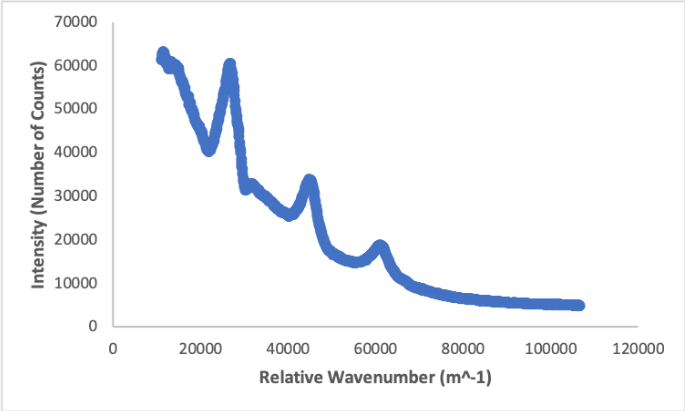
\includegraphics[width=0.48\textwidth]{Figures/PHYS 331 RS TiO2 Anti-Stokes Relative Wavenumber (4 Sec).png}
\caption{Anti-Stokes intensities of TiO2 at 4 second exposure. The first peak that occurred which is $\approx 26,000$  m$^{-1}$ can be neglected due to errors in the instruments of the experiment.}
\end{figure}
\newline
The "$\#$" in the Table 1 and the following Tables depict the counts that are proportional to the number of photons observed in the exposure interval.
%---------------------------------------------------------------------------
%	Table 1
%---------------------------------------------------------------------------
\begin{table}[htb]
\begin{center}
\begin{tabular}{|c|c|}
    \hline \textbf{Relative $\nu$ (m$^{-1}$)} & \textbf{Intensity \#} \\ \hline
    26,336 & 67,916 $\pm 6,686$ \\ \hline
    44,854 & 32,530 $\pm 3,203$ \\ \hline
    60,872 & 16,548 $\pm 1,629$ \\ \hline
\end{tabular}
\caption{\small{Anti-Stokes intensities of TiO2 at 4 second exposure.}}
\end{center}
\label{default}
\end{table}%
\newline
Figure 1 and Table 1 depict the results for a four second run of the anti-Stokes intensities. The intensities found in Table 1 were calculated with the use of a peak fitting software called Fityk. To calculate the intensities of the peaks, Fityk calculated the area under the curve for each individual peak. The relative wavenumber on the other hand was able to be calculated with first finding the wavelength of the peak with excel, and then converting it to a wavenumber, the laser's wavenumber was then subtracted off this value to give the relative wavenumber of the sample. Figure 2 shows the Stokes intensities of Titanium dioxide at a four second exposure.
%---------------------------------------------------------------------------
%	Figure 2
%---------------------------------------------------------------------------
\begin{figure}[htb]
\centering
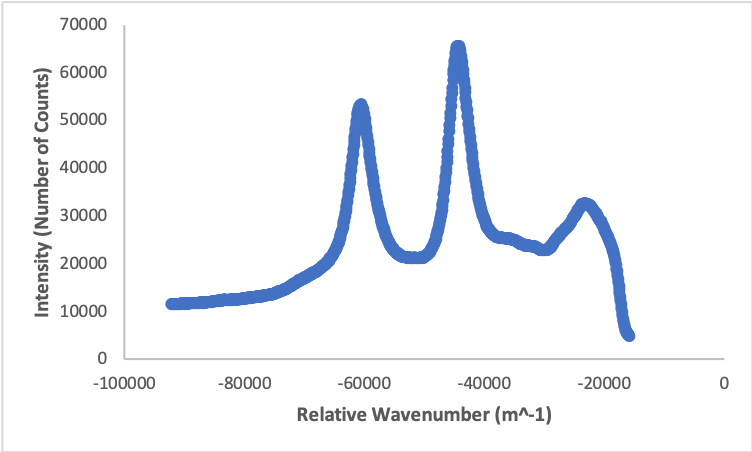
\includegraphics[width=0.48\textwidth]{Figures/PHYS 331 RS TiO2 Stokes Relative Wavenumber (4 Sec).png}
\caption{Stokes intensities of TiO2 at 4 second exposure.}
\label{s_ti_2sec}
\end{figure}
\newline
Figure 2 shows the Stokes intensities of TiO2 at three different relative wavenumbers. It should be noted that the relative wavenumbers are close to those found in the anti-Stokes plot in Figure 1. To better represent the Stokes intensities for TiO2 at the two second exposure Table 2 is constructed. The error in measurement for the intensity of the Stokes side was calculated to be $\approx 4.8\%$.
%---------------------------------------------------------------------------
%	Table 2
%---------------------------------------------------------------------------
\begin{table}[htb]
\begin{center}
\begin{tabular}{|c|c|}
    \hline \textbf{Relative $\nu$ (m$^{-1}$)} & \textbf{Intensity \#} \\ \hline
    -60,440 & 101,796 $\pm 4,881$ \\ \hline
    -44,176 & 128,282 $\pm 6,151$ \\ \hline
    -23,103 & 51,558 $\pm 2,472$ \\ \hline
\end{tabular}
\caption{Stokes intensities of TiO2 at 4 second exposure.}
\end{center}
\label{default}
\end{table}%
\newline
The intensities in Table 2 were calculated with a PsuedovoigtA function in Fityk where as the intensities in Table 1 were calculated with a GaussianA function. The choices of functions depended primarily on the shape of the peaks. In Figure 2, the peaks tend to be symmetric except for the last peak found around $\approx 23,000$ m$^{-1}$. Because of this odd shape of the last peak, the PsuedovoigtA function had to be used instead of the GaussianA function.

The Sulfur sample was examined at three seconds with the same procedure that was used for the Titanium dioxide. Figure 3 shows the anti-Stokes intensities for Sulfur at the three second exposure.
%---------------------------------------------------------------------------
%	Figure 3
%---------------------------------------------------------------------------
\begin{figure}[htbp]
\begin{center}
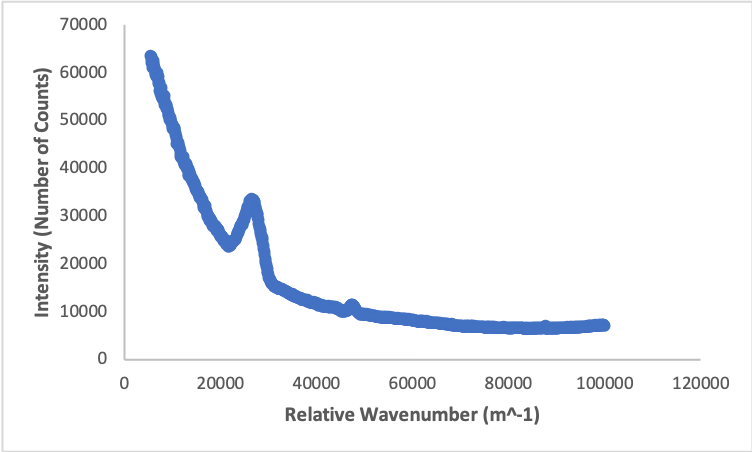
\includegraphics[width=0.48\textwidth]{Figures/PHYS 331 RS S Anti-Stokes Relative Wavenumber.png}
\caption{Anti-Stokes intensities of sulfur at 3 second exposure.}
\label{default}
\end{center}
\end{figure}
\newline
Figure 3 shows two distinct Raman peaks unlike the three Raman peaks that kept occurring in both Figure 1 and Figure 2 for the Titanium dioxide sample. The two samples share similar shapes for the anti-Stokes side of their respective room temperature Raman spectrums. The intensities and relative wavenumbers for each sample however are both different. The error in measurement of the intensities for the anti-Stokes side of Sulfur were different for each respective peak.  The peak that is $\approx 47,000$ m$^{-1}$ has an error of $\approx 9.98\%$ where as the peak that is $\approx 26,000$ m$^{-1}$ has an error of $\approx 1.08\%$. Table 3 is constructed to help convey the results seen in Figure 3. 
%---------------------------------------------------------------------------
%	Table 3
%---------------------------------------------------------------------------
\begin{table}[htp]
\begin{center}
\begin{tabular}{|c|c|}
    \hline \textbf{Relative $\nu$ (m$^{-1}$)} & \textbf{Intensity \#} \\ \hline
    26,336 & 45,386 $\pm 490$ \\ \hline
    47,468 & 2,014 $\pm 201$ \\ \hline
\end{tabular}
\caption{Anti-Stokes intensities of Sulfur at 3 second exposure.}
\end{center}
\label{default}
\end{table}%
\newline
First glance reveals that the larger peak (Meaning a greater area) has a smaller relative error and the smaller peak has a greater one. After the anti-Stokes intensities were examined the Stokes intensities were examined next which can be seen in Figure 4 below.
%---------------------------------------------------------------------------
%	Figure 4
%---------------------------------------------------------------------------
\begin{figure}[htbp]
\begin{center}
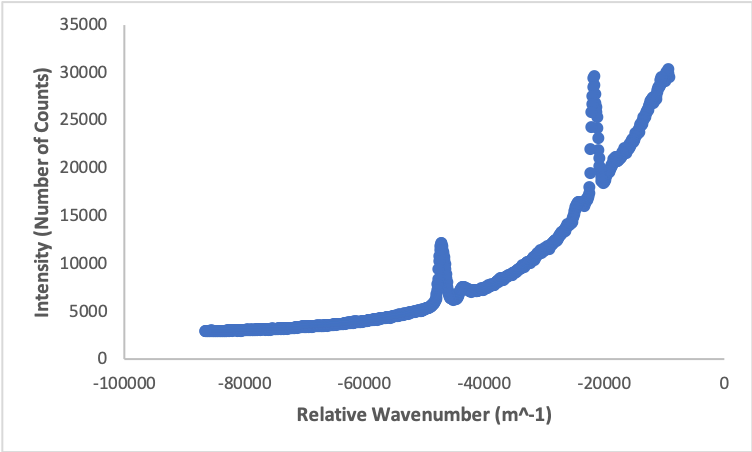
\includegraphics[width=0.48\textwidth]{Figures/PHYS 331 RS S Stokes Relative Wavenumber.png}
\caption{Stokes intensities of Sulfur at 3 second exposure. Smaller peaks that subside around the larger ones were neglected in the measurements for this side of 
Sulfur's room temperature Raman spectrum.}
\label{default}
\end{center}
\end{figure}
\newline
There are two distinct Raman peaks that occur on the Stokes side of Sulfur's Raman spectrum. Opposite of the anti-Stokes side, the uncertainties in the Stokes intensities were less for each individual peak. The first peak that occurs at $\approx -47,000$ m$^{-1}$ has an error of $\approx 1.46\%$. The second peak at $\approx -21,000$ m$^{-1}$ has an error of $\approx 1.52\%$. These two peaks can be seen in Table 4 below.
%---------------------------------------------------------------------------
%	Table 4
%---------------------------------------------------------------------------
\begin{table}[htp]
\begin{center}
\begin{tabular}{|c|c|}
    \hline \textbf{Relative $\nu$ (m$^{-1}$)} & \textbf{Intensity \#} \\ \hline
    -47,042 & 5,905 $\pm 86$ \\ \hline
    -21,694 & 8,643 $\pm 93$ \\ \hline
\end{tabular}
\caption{Stokes intensities of Sulfur at 3 second exposure.}
\end{center}
\label{default}
\end{table}%
\newline
The intensities in Figure 4 can be seen to have narrow peaks. These narrow peaks are a cause in why we see a smaller intensity value for the Stokes intensities of Sulfur compared to the anti-Stokes intensities.

The temperature of a sample can be calculated via the techniques that have been used in this lab surrounding Raman spectroscopy. In essence, we are calculating the temperature of the Titanium dioxide sample, not the room temperature. But since the sample is being stored at room temperature during the duration of this experiment, we can assume that the temperature of the sample is also the temperature of the room. For more information on how temperature affects the Raman spectrum of a material see reference [8] or [12]. The equation that is used to calculate the temperature of the sample is 
%---------------------------------------------------------------------------
%	Equation 1
%---------------------------------------------------------------------------
\begin{equation}\label{1}
	T=\frac{-h\cdot V_{\nu}}{k\cdot\ln{[\frac{(V_{l}-V_{\nu})^{3}}{(V_{l}+V_{\nu})^{3}}\cdot\frac{I_{AS}}{I_{S}}}]}
\end{equation}
where $h$ is Planck's constant, $k$ is Boltzman's constant, $V_{\nu}$ is the vibrational mode of the sample, $V_{l}$ is the vibrational mode of the laser, $I_{AS}$ is the intensity of the anti-Stokes, and $I_{S}$ is the intensity of the Stokes [8]. In the context of this experiment, the only variables that changes throughout each new run for Titanium dioxide is $V_{\nu}$, $I_{AS}$, and $I_{S}$. It is because of the majority of the variables not changing that we were able to get multiple measurements of temperature from the Titanium dioxide sample. Table 5 was constructed to depict the temperature estimates from the relative wavenumbers that were found for the anti-Stokes intensities of Titanium dioxide.
%---------------------------------------------------------------------------
%	Table 5
%---------------------------------------------------------------------------
\begin{table}[htp]
\begin{center}
\begin{tabular}{|c|c|c|}
	\hline \textbf{Relative $\nu$ (m$^{-1}$)} & \textbf{Intensity \#} & \textbf{Temp. (K)} \\ \hline
	26,336 & 67,916 & -2,365 $\pm$ 272 \\ \hline
	44,854 & 32,530 & 385 $\pm$ 44 \\ \hline
	60,872 & 16,548 & 394 $\pm$ 45 \\ \hline
\end{tabular}
\caption{Temperature estimates from Titanium dioxide for anti-Stokes intensities.}
\end{center}
\label{default}
\end{table}%
\newline
Immediate observations show that the peak with a relative wavenumber of $26,336$ m$^{-1}$ has a temperature estimate that cannot be accurate. Absolute zero is defined to be lowest temperature possible [10]. Absolute zero has never been reached according to all human observations to this date, and thus is why the temperature found for the relative wavenumber of Titanium dioxide of $-2,365 \pm 272$ K cannot be correct due to it being theoretically impossible. The other two measurements seen in Table 5, albeit they are not consistent with what room temperature is defined to be $\approx$ 293 K [6], they are both at least theoretically possible. The same analysis was ran for the Stokes intensities of Titanium dioxide and the temperature estimates can be seen in Table 6 below.
%---------------------------------------------------------------------------
%	Table 6
%---------------------------------------------------------------------------
\begin{table}[htp]
\begin{center}
\begin{tabular}{|c|c|c|}
	\hline \textbf{Relative $\nu$ (m$^{-1}$)} & \textbf{Intensity \#} & \textbf{Temp. (K)} \\ \hline
	-60,440 & 101,796 & 391 $\pm$ 45 \\ \hline
	-44,176 & 128,282 & 380 $\pm$ 44 \\ \hline
	-23,103 & 51,558 & -1,885 $\pm$ 217 \\ \hline
\end{tabular}
\caption{Temperature estimates from Titanium dioxide for Stokes intensities.}
\end{center}
\label{default}
\end{table}%
\newline
This time in Table 6 the relative wavenumber of $-23,103$ m$^{-1}$ has an impossible temperature estimate similar to the one in Table 5 of similar relative wavenumber. The other two temperature estimates in Table 6 are realistic temperatures, just not for room temperature. 

The last bit of information that is worth reporting are the overall ratios of the anti-Stokes to Stokes intensities of both the Titanium dioxide and Sulfur sample. The ratio for the anti-Stokes to Stokes intensity for the Titanium dioxide sample is 
%---------------------------------------------------------------------------
%	Equation 2
%---------------------------------------------------------------------------
\begin{equation}\label{2}
	\frac{I_{AS}}{I_{S}}=0.208 \pm 0.045.
\end{equation}
The value found in (2) was calculated with the intensities of the peaks found in both Table 1 and Table 2. The peak that was generating a temperature estimate that was not theoretically possible was not incorporated into the ratio calculation since this peak is more than likely an error from the instrumentation. From (2), the anti-Stokes to Stokes intensity ratio for Sulfur was found to be
%---------------------------------------------------------------------------
%	Equation 3
%---------------------------------------------------------------------------
\begin{equation}
	\frac{I_{AS}}{I_{S}}=0.420 \pm 0.070.
\end{equation}
Immediate inspection shows that the ratio of the anti-Stokes to Stokes intensity is greater for Sulfur than that of Titanium dioxide.
%---------------------------------------------------------------------------
%	Conclusions
%---------------------------------------------------------------------------
\section*{Conclusions}
Titanium dioxide and Sulfur's room temperature Raman spectrum were both observed with the intention to find a ratio of the anti-Stokes to Stokes intensities. From the calculated anti-Stokes to Stokes ratio, the room temperature was then calculated with the use equation (1). The best temperature estimate that was found amongst the data was $T=380\pm44$ K. Albeit $T=380\pm44$ K was the best measurement that was made in this experiment, it is not a correct value for the room temperature where this experiment was conducted. At it's lowest value of $T=336$ K, the temperature estimate is still 43 K away from a reasonable estimate for room temperature [6]. This discrepancy in temperature shows that the error found is due to systematic error. The biggest contributing factor to why the temperature estimate is so incorrect is more than likely due to the spectrometer or some other device in the instrumentation setup that needs to be calibrated. These modifications could lead to a better intensity measurement and thus a better estimate for the room temperature. It should be noted that the temperature estimate became closer to actual room temperature when the exposure time was increased. If this experiment were to be conducted again, a calibration amongst the equipment would be the primary issue to resolve, and then an exposure time longer than four seconds for either sample would be recommended.
%---------------------------------------------------------------------------
%	Bibliography
%---------------------------------------------------------------------------
\newpage
\begin{thebibliography}{12}
\bibitem{araujo}
Alene Silva Melo Ara\'ujo, Paula Ramalho Franca Flores, Victor Pinheiro Feitosa, L\'idia Audrey Rocha Valadas, Diego Martins de Paula, Nicole de Mello Fiallos, Igor Ribeiro Rola, Jos\'e Antero Soares Rola, Ana Cristina de Mello Fiallos. Micro-Raman Spectroscopy, Colour Stability, Roughness and Mass Variation of Removable Partial Dentures After Cleansing With White Wine Vinegar. Peer Reviewed. Fortaleza: Journal of Young Pharmacists, 2018.
\bibitem{chemistry}
Chemistry, Royal Society of. Periodic Table . 8 March 2019. March 2019. \url{http://www.rsc.org/periodic-table/element/16/sulfur}.
\bibitem{safety}
Facts, Chemical Safey. Chemical Safety Facts. 1 March 2019. March 2019. \url{https://www.chemicalsafetyfacts.org/titanium-dioxide/}.
\bibitem{meiid}
Gaoxiang MeiID, Natalia Mamaeva, Srividya Ganapathy , Peng Wang , Willem J. DeGrip2, Kenneth J. RothschildI. Raman Spectroscopy of a Near Infrared Absorbing Proteorhodopsin: Similarities to the Bacteriorhodopsin O Photointermediate. Peer Reviewed. Boston: PLOS ONE, 2018.
\bibitem{itoid}
Hiroaki ItoID, Naoyuki Uragami, Tomokazu Miyazaki, Noboru Yokoyama, Haruhiro Inoue. Raman Spectroscopic Evaluation of Human Serum Using Metal Plate and 785- nm and 1064- nm Excitation Lasers. Peer Reviewed. Koto: PLOS ONE, 2018.
\bibitem{nist}
NIST. NIST. 13 September 2018. March 2019. \url{https://www.nist.gov/pml/weights-and-measures/si-units-temperature}.
\bibitem{garbacz}
Patrycja Garbacz, Marek Wesolowski. DSC, FTIR and Raman Spectroscopy Coupled with Multivariate Analysis in a Study of Co-Crystals of Pharmaceutical Interest. Peer Reviewed. Gdansk: MDPI, 2018.
\bibitem{Tuschel}
Tuschel, David. Spectroscopy Online. 1 December 2016. March 2019. <http://www.spectroscopyonline.com/raman-thermometry>.
\bibitem{wiki_raman}
Wikipedia. Wikipedia. 31 January 2019. 16 February 2019. \url{https://en.Wikipedia.org/wiki/Raman_scattering}.
\bibitem{wiki_zero}
Wikipedia. Wikipedia. 9 March 2019. 10 March 2019. \url{https://en.wikipedia.org/wiki/Absolute_zero}.
\bibitem{zhang}
Yong Zhang, Jingjing Xu, Yuezhou Yu, Wenhao Shang, Anpei Ye. Anti-Cancer Drug Sensitivity Assay with Quantitative Heterogeneity Testing Using Single-Cell Raman Spectroscopy. Peer Reviewed. Beijing: MDPI, 2018
\bibitem{zzhang}
Zheng-Yong Zhang, Dong-Dong Gui, Min Sha, Jun Liu, Hai-Yan Wang. Raman Chemical Feature Extraction for Quality Control of Dairy Products. Peer Reviewed. Zhejiang: American Dairy Science Association, 2019.
\end{thebibliography}
\end{document}
